\chapter{Performance}

In systems programming, performance is a key metric for evaluating software efficiency, making the choice of programming language especially important. Rust promises zero-cost abstractions and performance comparable to C++, while also offering memory safety and fearless concurrency. To examine these claims, we developed separate tests for individual language features and measured their execution times.

\section{Comparing Code Performance in Rust vs C++}

In systems programming, performance is a key metric for evaluating software efficiency, making the choice of programming language especially important. Rust promises zero-cost abstractions and performance comparable to C++, while also offering memory safety and fearless concurrency. To examine these claims, we developed separate tests for individual language features and measured their execution times.

We implemented dedicated tests using Google’s Benchmark \cite[]{GoogleBenchmark2025} library for C++ and Criterion.rs \cite[]{heislerBheislerCriterionrs2025} for Rust. Specifically, we designed distinct tests for various features, including sorting (using each language’s standard sort function), closures (using Rust’s closures and the equivalent C++ lambda functions), memory allocation and management, and iterator operations. Each test was executed individually in comparable environments to evaluate the performance of each feature. We show our findings in Figure~\ref{fig:table1}.

\begin{figure}[htbp]
    \centering
    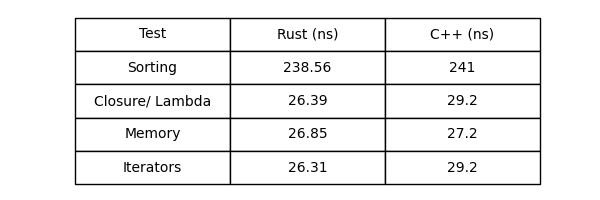
\includegraphics[width=0.8\textwidth]{images/table_1.png}
    \caption{Comparison of Execution speed of similar Rust and C++ feature implementations}
    \label{fig:table1}
\end{figure}

The results indicate that Rust and C++ deliver nearly identical execution times for each test, demonstrating that both Rust’s zero-cost abstractions and C++’s zero-overhead design compile to highly optimized code.

\paragraph{}

According to the study "Rewrite it in Rust: A Computational Physics Case Study"\cite{veytsmanRewriteItRust2024}, Veytsman et al.\ implement a physics simulation in Rust and C++ to analyze the performance difference between both implementations. The Rust implementation was based off of the C++ code, but made use of Rust's modules, closures and iterators. Their results when comparing both sequential implementations runtime, found that their Rust implementation (4.098s) was 1.6x as fast as their C++ implementation (7.521s). The study also included a parallelized implementation using Rust's Rayon library \cite[]{RayonrsRayon2025}. This resulted in a runtime performance gain of around 5.6x when comparing C++(487.63s) and Rust (146.939s). This however is an unfair comparison as C++ has various parallelization libraries that could have been used. It does however show that parallel Rust can be written easily and safely \cite{veytsmanRewriteItRust2024}.

\paragraph{}

Analyzing a study by J. Rotter and M. C. Lewis on comparing Rust to other languages in an N-Body benchmark. The benchmarks revealed that Rust and C++ had comparable performance, with Rust beating out C++ at higher particle count.

\begin{table}[h]
    \centering
    \begin{tabular}{|c|c|c|c|c|}
        \hline
        & \multicolumn{4}{|c|}{Number of Particles} \\  
        \hline
        Language & 1000 & 10000 & 100000 & 1000000 \\
        \hline
        Rust & 0.57 ± 0.01 & 11.52 ± 0.05 & 198 ± 2 & 2960 ± 50 \\
        C++ & 0.48 ± 0.02 & 10.07 ± 0.05 & 181 ± 6 & 3820 ± 30 \\
        C & 0.50 ± 0.01 & 10.17 ± 0.02 & 176 ± 3 & 3770 ± 10 \\
        \hline
    \end{tabular}
    \caption{Timing Results Between Rust, C++ and C according to Table 1 in \cite[]{rotterNBodyPerformanceKDTree2022} (lower is better)}
    \label{tab:performance_1}
\end{table}

Furthermore, the study analyzed the memory usage of the benchmark across the language. The findings showed that Rust used consistently less memory than C++ across all particle counts, coming very close to native C.

\begin{table}[h]
    \centering
    \begin{tabular}{|c|c|c|c|c|}
        \hline
        & \multicolumn{4}{|c|}{Number of Particles} \\  
        \hline
        Language & 1000 & 10000 & 100000 & 1000000 \\
        \hline
        Rust & 2.8 & 4.0 & 16 & 153 \\
        C++ & 3.8 & 5.7 & 19 & 202 \\
        C & 2.3 & 3.2 & 15.5 & 153 \\
        \hline
    \end{tabular}
    \caption{Resident Memory Usage in MB Between Rust, C++ and C according to Table 2 in \cite[]{rotterNBodyPerformanceKDTree2022} (lower is better)}
    \label{tab:performance_2}
\end{table}